% -*- coding: utf-8 -*-
%-------------------------designed by zcf--------------
\documentclass[UTF8,a4paper,10pt]{ctexart}
\usepackage[left=3.17cm, right=3.17cm, top=2.74cm, bottom=2.74cm]{geometry}
\usepackage{amsmath}
\usepackage{graphicx,subfig}
\usepackage{float}
\usepackage{cite}
\usepackage{caption}
\usepackage{enumerate}
\usepackage{booktabs} %表格
\usepackage{multirow}
\newcommand{\tabincell}[2]{\begin{tabular}{@{}#1@{}}#2\end{tabular}}  %表格强制换行
%-------------------------字体设置--------------
% \usepackage{times} 
\usepackage{ctex}
\setCJKmainfont[ItalicFont=Noto Sans CJK SC Bold, BoldFont=Noto Serif CJK SC Black]{Noto Serif CJK SC}

\newcommand{\yihao}{\fontsize{26pt}{36pt}\selectfont}           % 一号, 1.4 倍行距
\newcommand{\erhao}{\fontsize{22pt}{28pt}\selectfont}          % 二号, 1.25倍行距
\newcommand{\xiaoer}{\fontsize{18pt}{18pt}\selectfont}          % 小二, 单倍行距
\newcommand{\sanhao}{\fontsize{16pt}{24pt}\selectfont}  %三号字
\newcommand{\xiaosan}{\fontsize{15pt}{22pt}\selectfont}        % 小三, 1.5倍行距
\newcommand{\sihao}{\fontsize{14pt}{21pt}\selectfont}            % 四号, 1.5 倍行距
\newcommand{\banxiaosi}{\fontsize{13pt}{19.5pt}\selectfont}    % 半小四, 1.5倍行距
\newcommand{\xiaosi}{\fontsize{12pt}{18pt}\selectfont}            % 小四, 1.5倍行距
\newcommand{\dawuhao}{\fontsize{11pt}{11pt}\selectfont}       % 大五号, 单倍行距
\newcommand{\wuhao}{\fontsize{10.5pt}{15.75pt}\selectfont}    % 五号, 单倍行距
%-------------------------章节名----------------
\usepackage{ctexcap} 
\CTEXsetup[name={,、},number={ \chinese{section}}]{section}
\CTEXsetup[name={(,)},number={\chinese{subsection}}]{subsection}
\CTEXsetup[name={,.},number={\arabic{subsubsection}}]{subsubsection}
%-------------------------页眉页脚--------------
\usepackage{fancyhdr}
\pagestyle{fancy}
\lhead{\kaishu \leftmark}
% \chead{}
\rhead{\kaishu 计算机网络实验报告}
\lfoot{}
\cfoot{\thepage}
\rfoot{}
\renewcommand{\headrulewidth}{0.1pt}  
\renewcommand{\footrulewidth}{0pt}%去掉横线
\newcommand{\HRule}{\rule{\linewidth}{0.5mm}}%标题横线
\newcommand{\HRulegrossa}{\rule{\linewidth}{1.2mm}}
%-----------------------伪代码------------------
\usepackage{algorithm}  
\usepackage{algorithmicx}  
\usepackage{algpseudocode}  
\floatname{algorithm}{Algorithm}  
\renewcommand{\algorithmicrequire}{\textbf{Input:}}  
\renewcommand{\algorithmicensure}{\textbf{Output:}} 
\usepackage{lipsum}  
\makeatletter
\newenvironment{breakablealgorithm}
  {% \begin{breakablealgorithm}
  \begin{center}
     \refstepcounter{algorithm}% New algorithm
     \hrule height.8pt depth0pt \kern2pt% \@fs@pre for \@fs@ruled
     \renewcommand{\caption}[2][\relax]{% Make a new \caption
      {\raggedright\textbf{\ALG@name~\thealgorithm} ##2\par}%
      \ifx\relax##1\relax % #1 is \relax
         \addcontentsline{loa}{algorithm}{\protect\numberline{\thealgorithm}##2}%
      \else % #1 is not \relax
         \addcontentsline{loa}{algorithm}{\protect\numberline{\thealgorithm}##1}%
      \fi
      \kern2pt\hrule\kern2pt
     }
  }{% \end{breakablealgorithm}
     \kern2pt\hrule\relax% \@fs@post for \@fs@ruled
  \end{center}
  }
\makeatother
%------------------------代码-------------------
\usepackage{xcolor} 
\usepackage{listings} 
\usepackage{graphicx}
\lstset{ 
breaklines,%自动换行
basicstyle=\small,
escapeinside=``,
keywordstyle=\color{ blue!70} \bfseries,
commentstyle=\color{red!50!green!50!blue!50},% 
stringstyle=\ttfamily,% 
extendedchars=false,% 
linewidth=\textwidth,% 
numbers=left,% 
numberstyle=\tiny \color{blue!50},% 
frame=trbl% 
rulesepcolor= \color{ red!20!green!20!blue!20} 
}
%------------超链接----------
\usepackage[colorlinks,linkcolor=black,anchorcolor=blue]{hyperref}
%------------------------TODO-------------------
\usepackage{enumitem,amssymb}
\newlist{todolist}{itemize}{2}
\setlist[todolist]{label=$\square$}
% for check symbol 
\usepackage{pifont}
\newcommand{\cmark}{\ding{51}}%
\newcommand{\xmark}{\ding{55}}%
\newcommand{\done}{\rlap{$\square$}{\raisebox{2pt}{\large\hspace{1pt}\cmark}}\hspace{-2.5pt}}
\newcommand{\wontfix}{\rlap{$\square$}{\large\hspace{1pt}\xmark}}
%------------------------水印-------------------
\usepackage{tikz}
\usepackage{xcolor}
\usepackage{eso-pic}
\usepackage{verbatim}

\newcommand{\watermark}[3]{\AddToShipoutPictureBG{
\parbox[b][\paperheight]{\paperwidth}{
\vfill%
\centering%
\tikz[remember picture, overlay]%
  \node [rotate = #1, scale = #2] at (current page.center)%
    {\textcolor{gray!80!cyan!30!magenta!30}{#3}};
\vfill}}}
\lstset{
  basicstyle=\ttfamily\small, % 使用打字机字体并设置为小号
  numbers=left,
}
%———————————————————————————————————————————正文
%----------------------------------------------
\begin{document}
\begin{titlepage}
    \begin{center}
    
\includegraphics[width=0.8\textwidth]{NKU.png}\\[1cm]    
    \textsc{\Huge \kaishu{\textbf{南\ \ \ \ \ \ 开\ \ \ \ \ \ 大\ \ \ \ \ \ 学}} }\\[0.9cm]
    \textsc{\huge \kaishu{\textbf{网\ \ 络\ \ 空\ \ 间\ \ 安\ \ 全\ \ 学\ \ 院}}}\\[0.9cm]
    \textsc{\huge \kaishu{\textbf{计算机网络实验报告}}}\\[0.8cm]
    \HRule \\[0.9cm]
    { \LARGE \bfseries Lab1 在线群聊程序}\\[0.4cm]
    \HRule \\[2.0cm]
    \centering
    \textsc{\LARGE \kaishu{2113946\ \ \ 刘国民 }}\\[0.5cm]
    \textsc{\LARGE \kaishu{年级\ :\ 2021级}}\\[0.5cm]
    \textsc{\LARGE \kaishu{专业\ :\ 信息安全}}\\[0.5cm]
    \vfill
    {\Large \today}
    \end{center}
\end{titlepage}



\newpage

\tableofcontents
\setcounter{page}{1}



\section{实验介绍}
本次实验基于C++中基本的Socket函数,通过多线程的方式,使用流式套接字实现了多人群聊的功能。该程序有基本的对话界面,输入"q"后可以正确退出程序。程序基本功能介绍:\par



\begin{itemize}
\item 进入用户端和服务端时,会输出相应的提示信息
\item 支持多人在线群聊,新的用户进入群聊后,会向其他用户提示进群的消息,同时提示新用户当前有哪些用户在线
\item 群聊时每个用户有自己的用户名,群聊时服务端会将发送时间、用户名和原始消息一起发送给其他用户
\item 服务端将历史聊天记录和用户进入/离开在线聊天室的信息显示在控制台上
\item 有用户退出在线群聊时,会告诉其他用户该用户已退出群聊,且不影响其他用户正常聊天
\item 发生错误时返回错误码
\end{itemize}

\section{协议设计}

\subsection{原理}


\subsubsection{套接字}

线程通过套接字发送消息和接收消息。主要包括以下两种类型:
\begin{itemize}
\item 数据报套接字:使用UDP协议,支持主机之间面向非连接、不可靠的数据传输
\item 流式套接字:使用TCP协议,支持主机之间面向连接的、顺序的、可靠的字节流传输
\end{itemize}

\subsubsection{协议}

网络协议是计算机网络中用于交换数据和进行通信的规定和标准。简单来说,它定义了两个或多个通信设备之间如何互相发送和接收数据的规则和约定。\par
以下为网络协议的组成要素:
\begin{itemize}
\item 语法:数据与控制信息的结构或格式(协议数据单元PDU)
\item 语义:需要发出何种控制信息,完成何种动作以及做出何种响应
\item 时序:事件实现顺序的详细说明
\end{itemize}

在SOCKET编程中,服务端和客户端通过SOCKET套接字来进行通信。按照Windows SOCKET API 提供的函数接口,符合语法规范和参数含义对函数进行调用。以下给出利用流式套接字通信的过程:
\begin{itemize}
\item 服务端/客户端通过SOCKET函数创建套接字,绑定传输层协议
\item 服务端/客户端通过bind函数将IP地址和端口与创建的套接字进行绑定
\item 客户端发送连接请求(connect)给服务端
\item 服务端监听(listen)到来的连接请求,返回新的套接字用于直接通信
\item 客户端发送(send)消息给服务端
\item 服务端接收(recv)发送的消息
\item 服务端/客户端断开(close)连接
\end{itemize}


\vspace{0.5cm}
本次实验中,一共有三种消息格式:
\begin{itemize}
\item 进入消息:以“\$n\$ame:”开头的消息,代表用户进入群聊,用这一消息告诉服务端用户名
\item 普通消息:time \ \ Name:Message,用于转发给其他用户。
\item 退出消息:即字符串q,代表用户退出群聊,用这一消息通知退出用户的子线程

\end{itemize}
\subsection{实现}
 按照实验要求和目标,本次实验采取以下协议设计方案:
\begin{itemize}
\item 使用TCP传输协议,选用流式套接字,采用多线程方式
\item 调用Socket函数时,输出错误码,便于调试程序
\item 设计两个源程序,$Server.cpp$ 和 $Client.cpp$。开启程序时需要首先打开$Server.exe$,再启动多个$Client.exe$。关闭时需要多个$Client.exe$正确退出(输入q退出),之后再关闭$Server.exe$,结束通信。
\end{itemize}


\section{设计思路}

\subsection{服务端}
首先进入服务端时,会输出提示语句。
服务端通过一个全局链表来维护当前成功和服务端连接的用户。链表节点包含用户的SOCKET套接字和用户名。

\subsubsection{主线程}
服务端的main函数负责打开WSA(Windows SOCKET API),进行服务端IP地址和端口号的初始化。调用socket返回套接字,并通过bind将套接字与服务端IP地址和端口进行绑定。之后调用listen函数持续监听到来的连接请求,如果成功accept到新的客户端请求,就为该客户创建新的线程AcceptThread,并且把Accept返回的新套接字传递给创建的线程,将用户信息插入到链表中。

\subsubsection{子线程}
服务端子线程如果成功accept到客户端,则输出“用户xxx成功连接的消息”。子线程中服务端通过recv来接收连接用户发送的消息。消息一共有三种类型:

\begin{itemize}
\item 客户端在用户成功与服务端连接后,会向服务端发送一条“\$n\$ame:”(这个奇怪的符号是为了避免与用户正常输入的消息相冲突)$+$用户名的消息,用于服务端设置新加入链表节点的用户名,同时将新加入的用户广播给其他用户,即:xx用户加入群聊,同时遍历链表中所有节点的用户名并发送给这个新加入的用户,告诉该用户目前群聊中有哪些用户在线。
\item 对于普通消息,即用户想发送给其他用户的消息。服务器只需遍历整个链表,跳过发送消息的用户,把当前时间、发送者的名字和消息相拼接,然后转发给其他用户。
\item 对于退出提示符“q”,需要通知客户端子线程,结束receive线程,客户端的ReceiveThread线程也需要用“q”来判别,如果客户端收到服务端发回的“q”,则通过return 0结束线程;同时需要从链表上删除该用户,表示该用户已下线;最后还需要把该用户退出的信息广播给其他用户。
\end{itemize}

\subsection{客户端}
进入客户端后与服务端类似,会输出提示语句。客户端主线程用于发送消息,线程用于接收服务端的消息。

\subsubsection{主线程}
客户端main函数首先完成WSAStartup、socket等初始化函数(这里不需要bind,因为操作系统会自动为客户端选择一个适当的IP和一个随机的临时端口号),之后通过cin.getline获取用户名,调用connect与服务端进行连接,连接成功后会输出提示信息,并且在这里会将“\$n\$ame:”和输入的用户名拼接后发给服务端,之后则创建线程ReceiveThread,用于接收服务端发送的消息,主线程则持续获取用户的输入,并且把内容发送给服务端,进而转发给其他用户。如果输入“q”,则会退出该群聊,结束主线程。

\subsubsection{子线程}
子线程用于接收服务端发来的消息,消息一共有两类:

\begin{itemize}
\item 其他用户发送给服务端的消息,服务端进而转发给除发送者外的所有用户,在这里得到消息后正常输出即可。
\item 用户自己发送给服务端的退出提示符“q”,服务端发回给用户自己,用于结束子线程。
\end{itemize}


\section{代码实现}
服务端和客户端的主线程实现较为简单,按照socket函数的调用语法,进行初始化即可。在此不再赘述,下面给出服务端和客户端子线程中的核心代码片段:
\subsection{服务端}
给出子线程收到三种类型消息的处理:\par
1、收到用户退出提示符q
\begin{lstlisting}[frame=trbl,language={C++}]
if (strcmp(Message, "q") == 0) {
    // 通知客户端子进程,结束receive
    if (SOCKET_ERROR == send(ClientSocket, Message, sizeof(Message), 0)) {
        cout << "send函数产生错误,具体错误信息见下:" << endl;
        cout << WSAGetLastError() << endl;
    }
    // 从链表上删除该客户端
    char ExitInfo[MAX_NAME_LEN+14] = { 0 };
    strcpy(ExitInfo, "用户");
    for (list<ClientInfo>::iterator curr = mylist.begin(); curr != mylist.end(); curr++) {
        if (curr->S_Client == ClientSocket) {
            cout << "用户" << curr->Name << "已断开连接!" << endl;
            strcat(ExitInfo,curr->Name);
            mylist.erase(curr);
            break;
        }
    }
    strcat(ExitInfo, "退出聊天!");
    // 广播给其他用户该用户已退出聊天
    for (list<ClientInfo>::iterator curr = mylist.begin(); curr != mylist.end(); curr++) {
        if (SOCKET_ERROR == send(curr->S_Client, ExitInfo, sizeof(ExitInfo), 0)) {
            cout << "send函数产生错误,具体错误信息见下:" << endl;
            cout << WSAGetLastError() << endl;
            WSACleanup();
            return 0;
        }
    }
    return 0; // 该用户已退出,结束该进程
}
\end{lstlisting}\par
消息q用于表明发送该消息的用户已经退出,为了确保聊天程序继续正常执行,需要结束服务端为该用户创建的Accept线程,即服务端把该用户正常消息广播出去的线程,还需要结束该用户自己的接收其他用户消息的线程。所以步骤如下:
\begin{itemize}
\item 把消息q发送回退出用户的客户端接受线程,通知其退出
\item 链表上删除该用户的节点
\item 服务端后台输出“用户xxx断开连接!”
\item 以socket为关键字遍历链表,把“用户xxx退出聊天!”广播给其他用户
\item return 0 结束该线程
\end{itemize}
2、收到前缀为\$n\$ame:的消息
\begin{lstlisting}[frame=trbl,language={C++}]
// Message是recv到的消息
string str(Message);
string pre = str.substr(0, 7);
if (pre == "$n$ame:") {     // 服务端设置用户名字
    strcpy(mylist.back().Name, Message + 7);// 在链表中存下名字
    cout << "用户" << mylist.back().Name << "成功建立连接!" << endl;

    char to_other[MAX_NAME_LEN+14] = { 0 };                // 将新加入的用户消息广播给其他用户
    char to_self[100] = { 0 };                             // 用于存储已在线的用户
    
    strcpy(to_other, "用户");
    strcat(to_other, mylist.back().Name);
    strcat(to_other, "加入聊天!");             // “用户xxx加入聊天”推送给其他用户
    strcpy(to_self, "当前在线用户:");

    list<ClientInfo>::iterator self = mylist.begin();
    for (list<ClientInfo>::iterator curr = mylist.begin(); curr != mylist.end(); curr++) {
        if (curr->S_Client != ClientSocket) { // 跳过发送消息的人
            if (SOCKET_ERROR == send(curr->S_Client, to_other, sizeof(to_other), 0)) {
                cout << "send函数产生错误,具体错误信息见下:" << endl;
                cout << WSAGetLastError() << endl;
                WSACleanup();
                return 0;
            }
        }
        else {
            self = curr;
        } 
        strcat(to_self, curr->Name);   // 加上用户的名字
        strcat(to_self, "  ");
    }
    // 发给新加入的用户to_self
    if (SOCKET_ERROR == send(self->S_Client, to_self, sizeof(to_self), 0)) {
        cout << "send函数产生错误,具体错误信息见下:" << endl;
        cout << WSAGetLastError() << endl;
        WSACleanup();
        return 0;
    }
    continue;
}
\end{lstlisting}\par
这类消息是成功连接的用户用来传输用户名字的特殊消息。处理步骤为:
\begin{itemize}
\item 服务端后台输出“用户xxx成功建立连接”的提示语
\item 根据socket套接字遍历所有成功连接的用户链表,把“用户xxx加入聊天的消息”广播给其他人
\item 遍历到新用户自身时用一个临时指针保存,之后把所有在线用户的用户名发送通过临时指针发送给新用户
\end{itemize}
3、普通消息
\begin{lstlisting}
char MessageInfo[MAX_MESSAGE_LEN + MAX_NAME_LEN + MAX_TIME_LEN + 2] = { 0 }; // MessageInfo = time  name:Message
strcpy(MessageInfo, GetTimeNow());
strcat(MessageInfo, "\n");
// 遍历链表,根据SOCKET找到发送者名字
for (list<ClientInfo>::iterator curr = mylist.begin(); curr != mylist.end(); curr++) {
    if (curr->S_Client == ClientSocket) {
        strcat(MessageInfo, curr->Name);
        break;
    }
}
strcat(MessageInfo, ":");
strcat(MessageInfo, Message);
cout << MessageInfo << endl;
// 对消息进行广播
for (list<ClientInfo>::iterator curr = mylist.begin(); curr != mylist.end(); curr++) {
    if (curr->S_Client != ClientSocket) { // 跳过发送消息的人
        if (SOCKET_ERROR == send(curr->S_Client, MessageInfo, sizeof(MessageInfo), 0)) {
            cout << "send函数产生错误,具体错误信息见下:" << endl;
            cout << WSAGetLastError() << endl;
            WSACleanup();
            return 0;
        }
    }
}

\end{lstlisting}\par
普通消息处理较为简单,只需根据Socket套接字从链表中找到发送用户的用户名,然后把时间和消息一起拼接后发送给其他用户。
\subsection{客户端}
给出子线程收到两种类型消息的处理:\par
\begin{lstlisting}
DWORD WINAPI ReceiveThread(LPVOID param) {                                               // 用来接收服务器发送的消息
    char ReceiveMessage[MAX_MESSAGE_LEN + MAX_NAME_LEN + MAX_TIME_LEN + 3] = { 0 };      // 名字最大长度和消息最大长度和冒号
    SOCKET ClientSocket = (SOCKET)param;                                                 // 类型转换,拿到主线程传递的参数
    while (true) {
        if (SOCKET_ERROR == recv(ClientSocket, ReceiveMessage, sizeof(ReceiveMessage), 0)) {
            cout << "receive接收失败" << endl;
            cout << WSAGetLastError() << endl;
            break;
        }
        if (strcmp(ReceiveMessage, "q") == 0) {                              // 客户输入q退出时,服务端会发送q到接收进程,关闭该进程
            return 0;
        }
        cout << ReceiveMessage << endl << endl;
    }
    return 0;// 正常退出
}
\end{lstlisting}\par
如上述设计思路所说,用户端的子线程用于接收两类消息:
\begin{itemize}
\item 其他用户发送给服务端的消息,服务端进而转发给除发送者外的所有用户,在这里得到消息后正常输出即可。
\item 用户自己发送给服务端的退出提示符“q”,服务端发回给用户自己,用于结束子线程。
\end{itemize}
所以在接收到消息后,如果是退出消息q,则直接return 0 结束线程,如果非q则为正常消息,直接输出即可。


\section{程序运行}
下面分析程序执行流程和通过WireShark捕获的消息

\subsection{流程分析}
如图,首先打开1个服务端程序和3个客户端程序
\begin{figure}[H]
    \centering
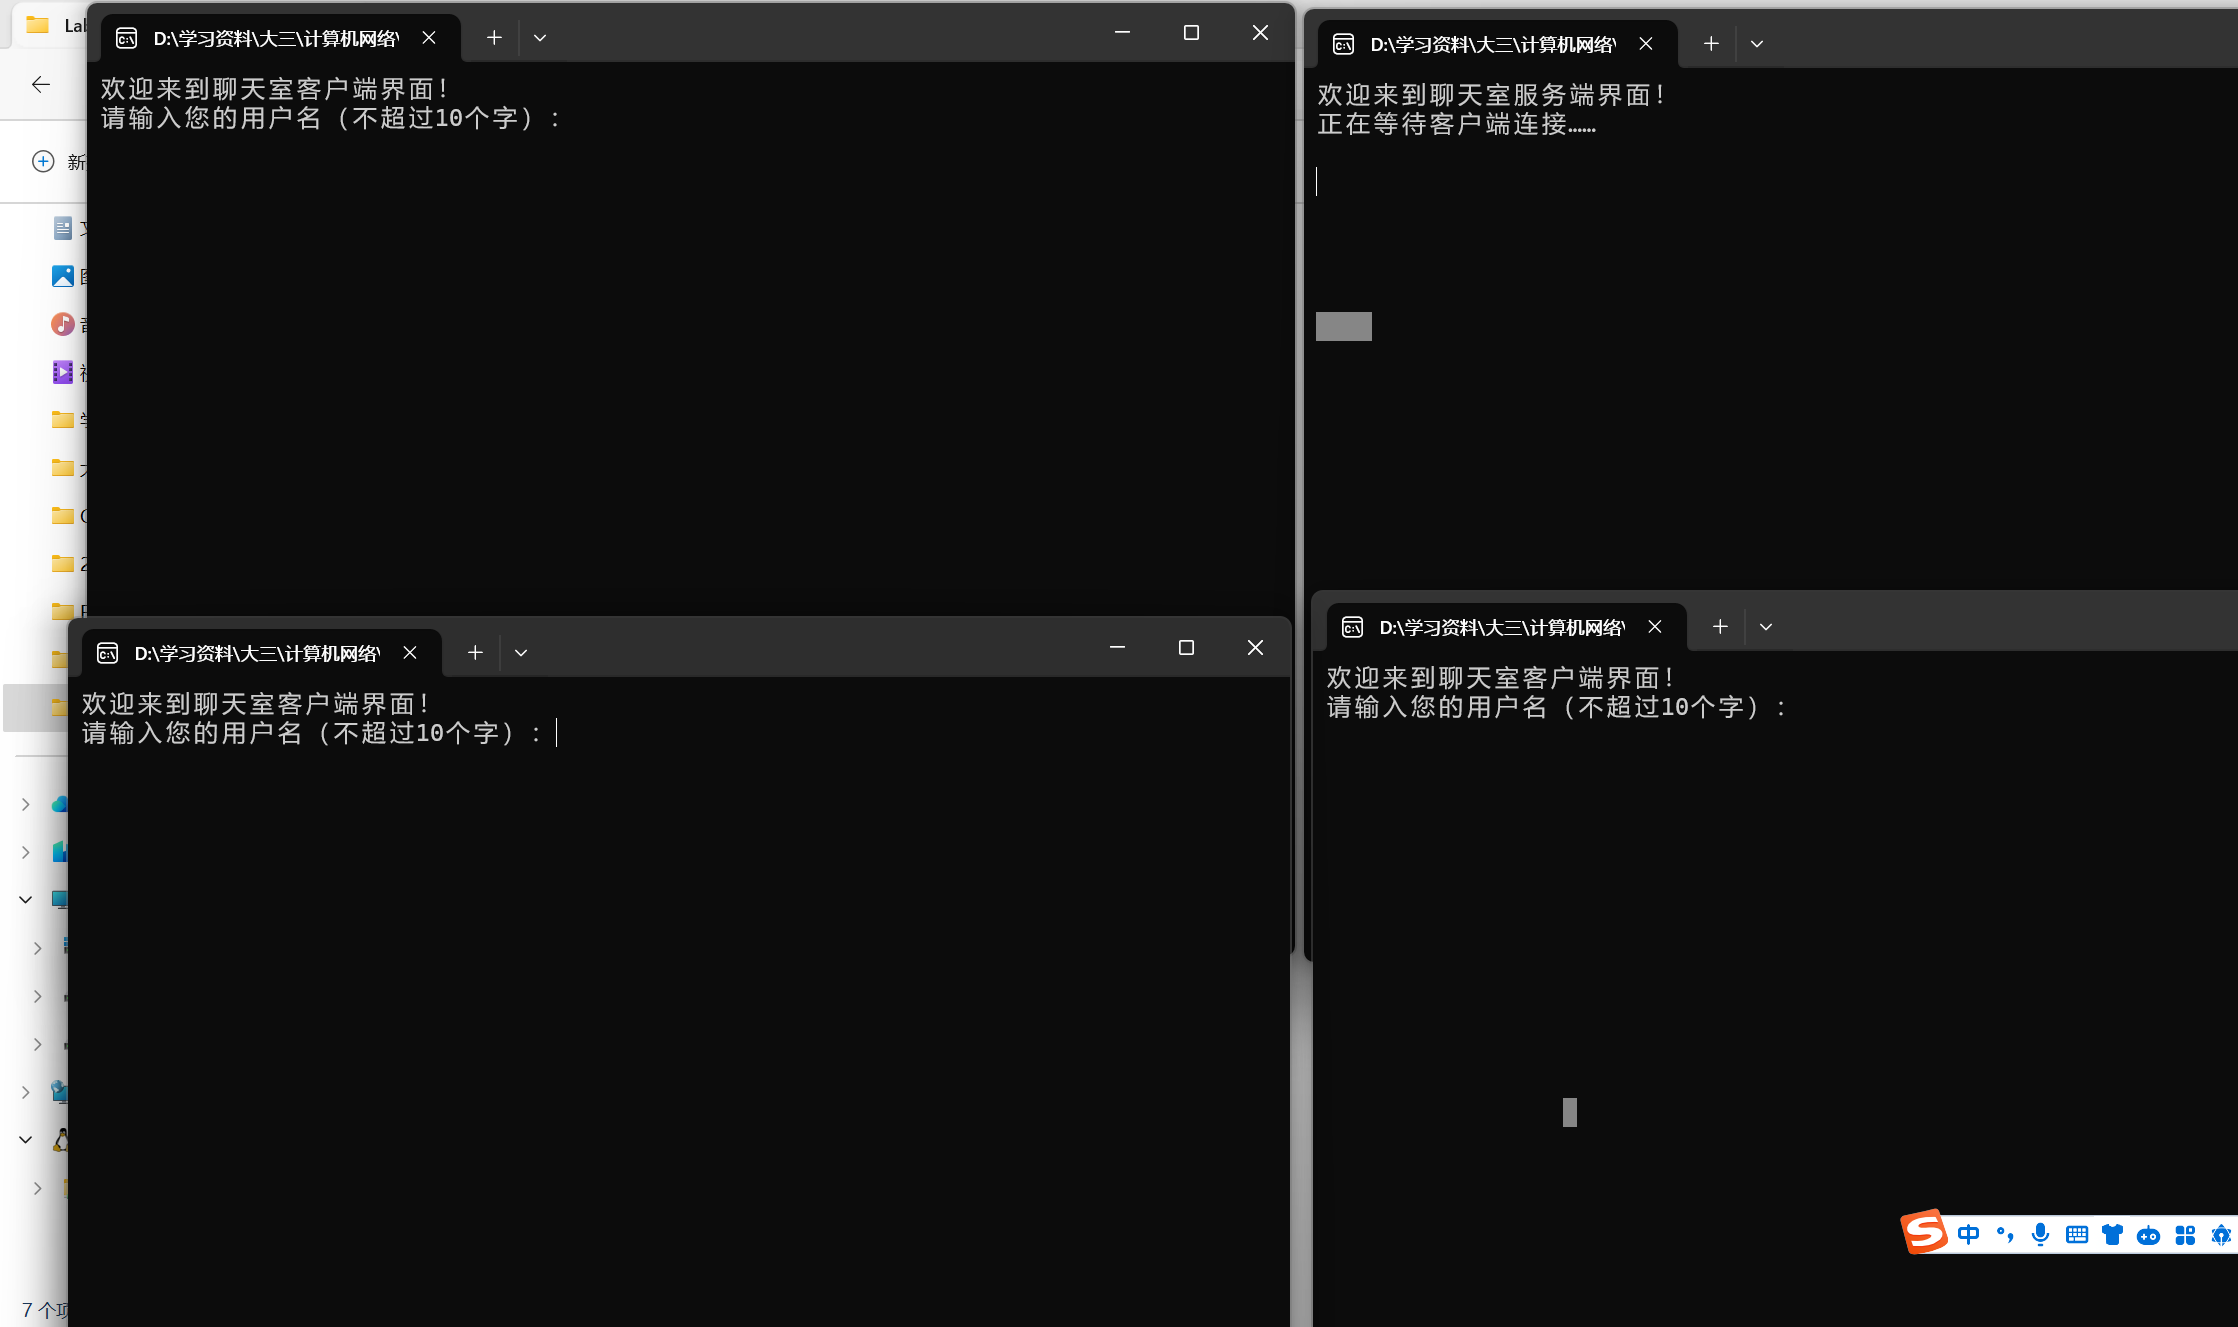
\includegraphics[width=0.8\textwidth]{img/初始化.png}
    \caption{初始化}
\end{figure}
然后按照NKU1-NKU2-NKU3的顺序输入用户名进入群聊,可以看到,其他用户进入时,已经在线的用户会收到通知
\begin{figure}[H]
    \centering
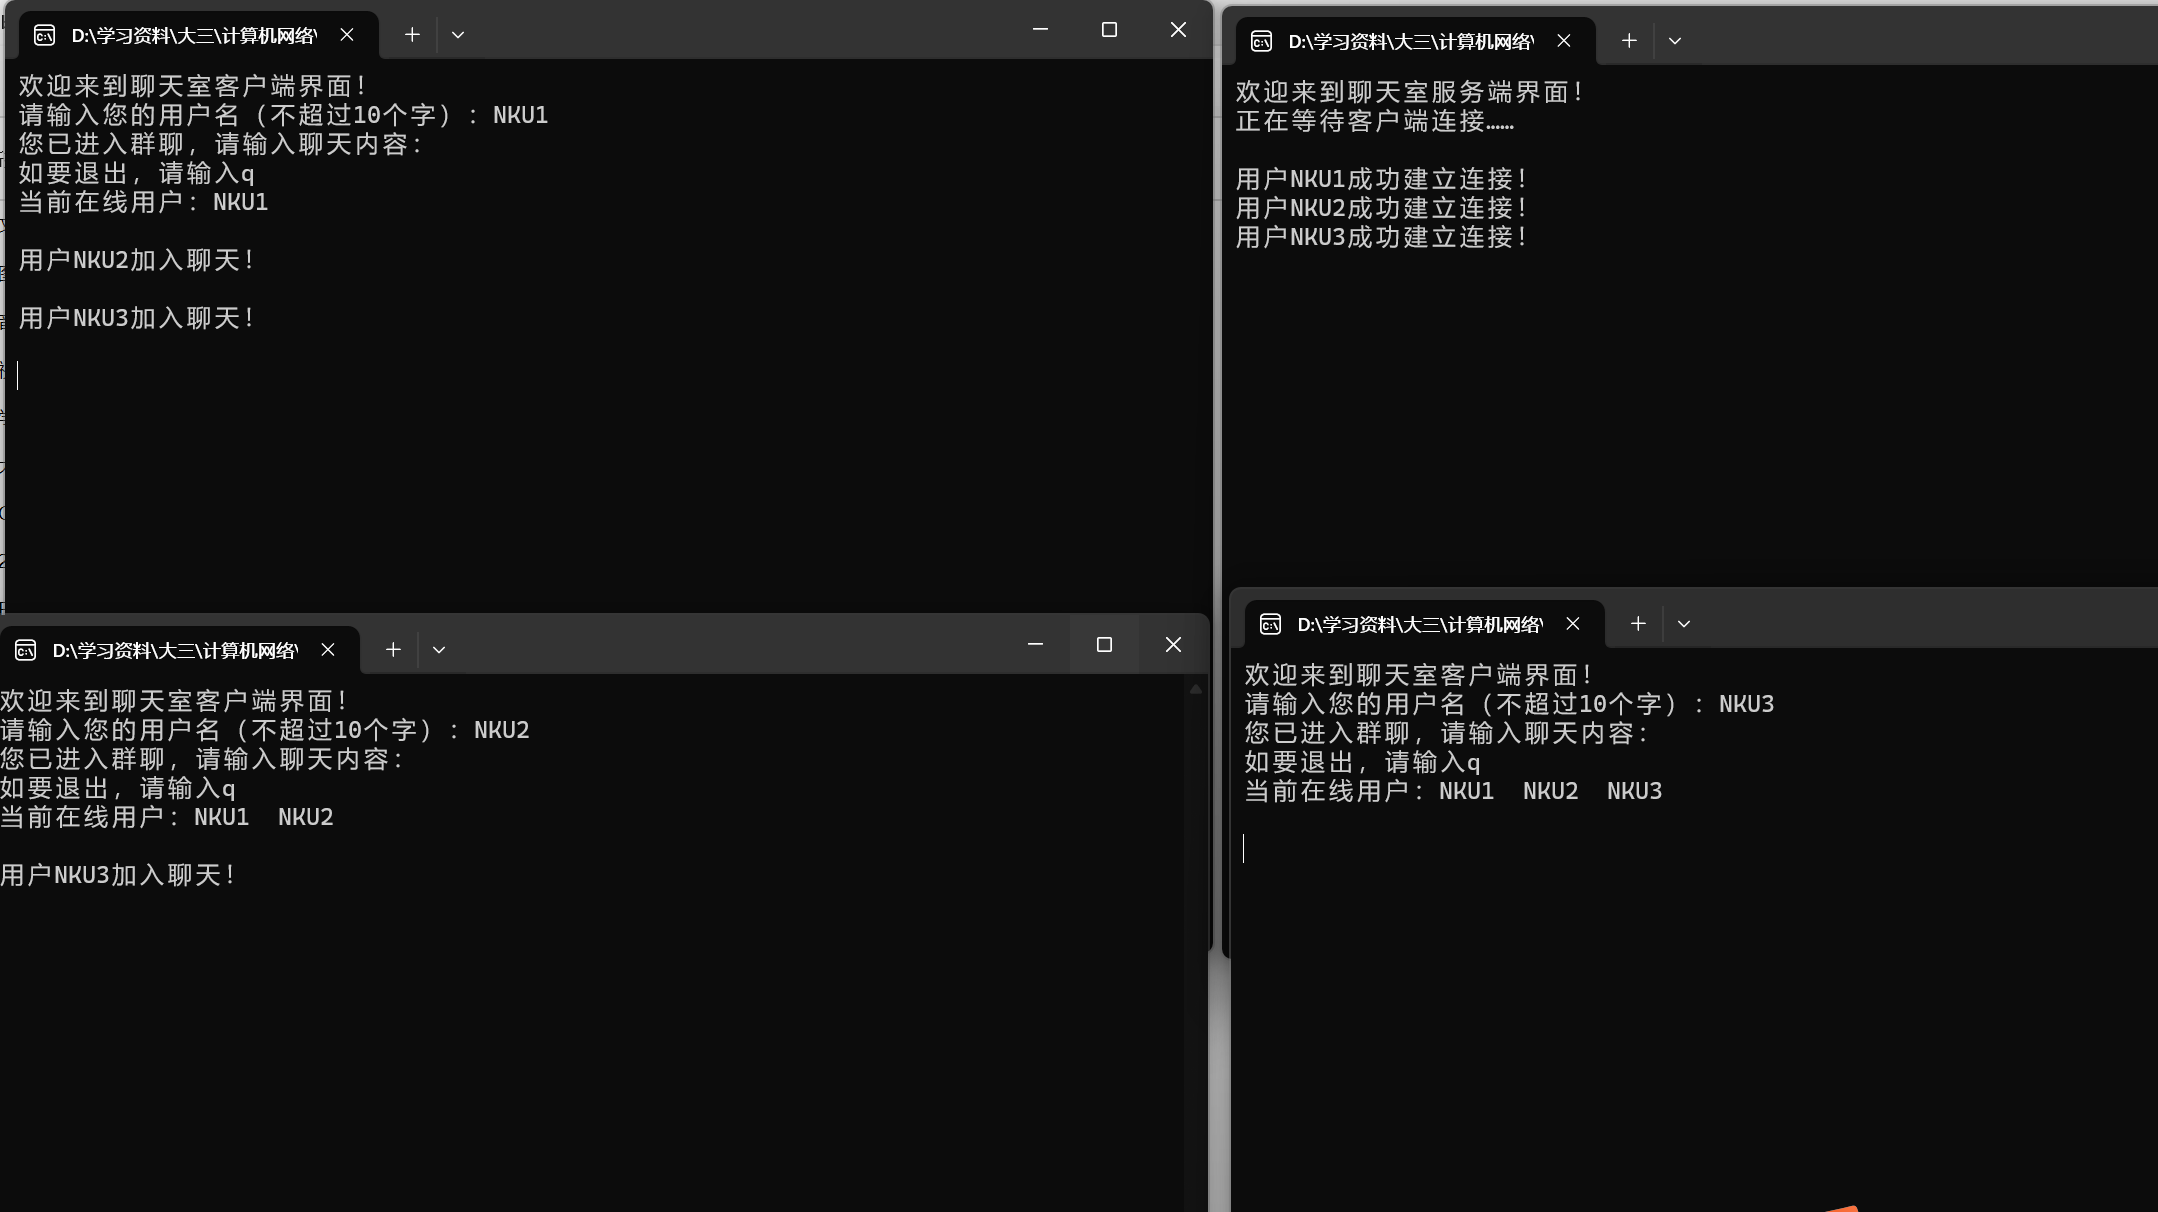
\includegraphics[width=0.8\textwidth]{img/进入群聊.png}
    \caption{进入群聊}
\end{figure}
之后开始发送消息,其他用户都可以正常收到消息,后台服务端正常输出聊天记录
\begin{figure}[H]
    \centering
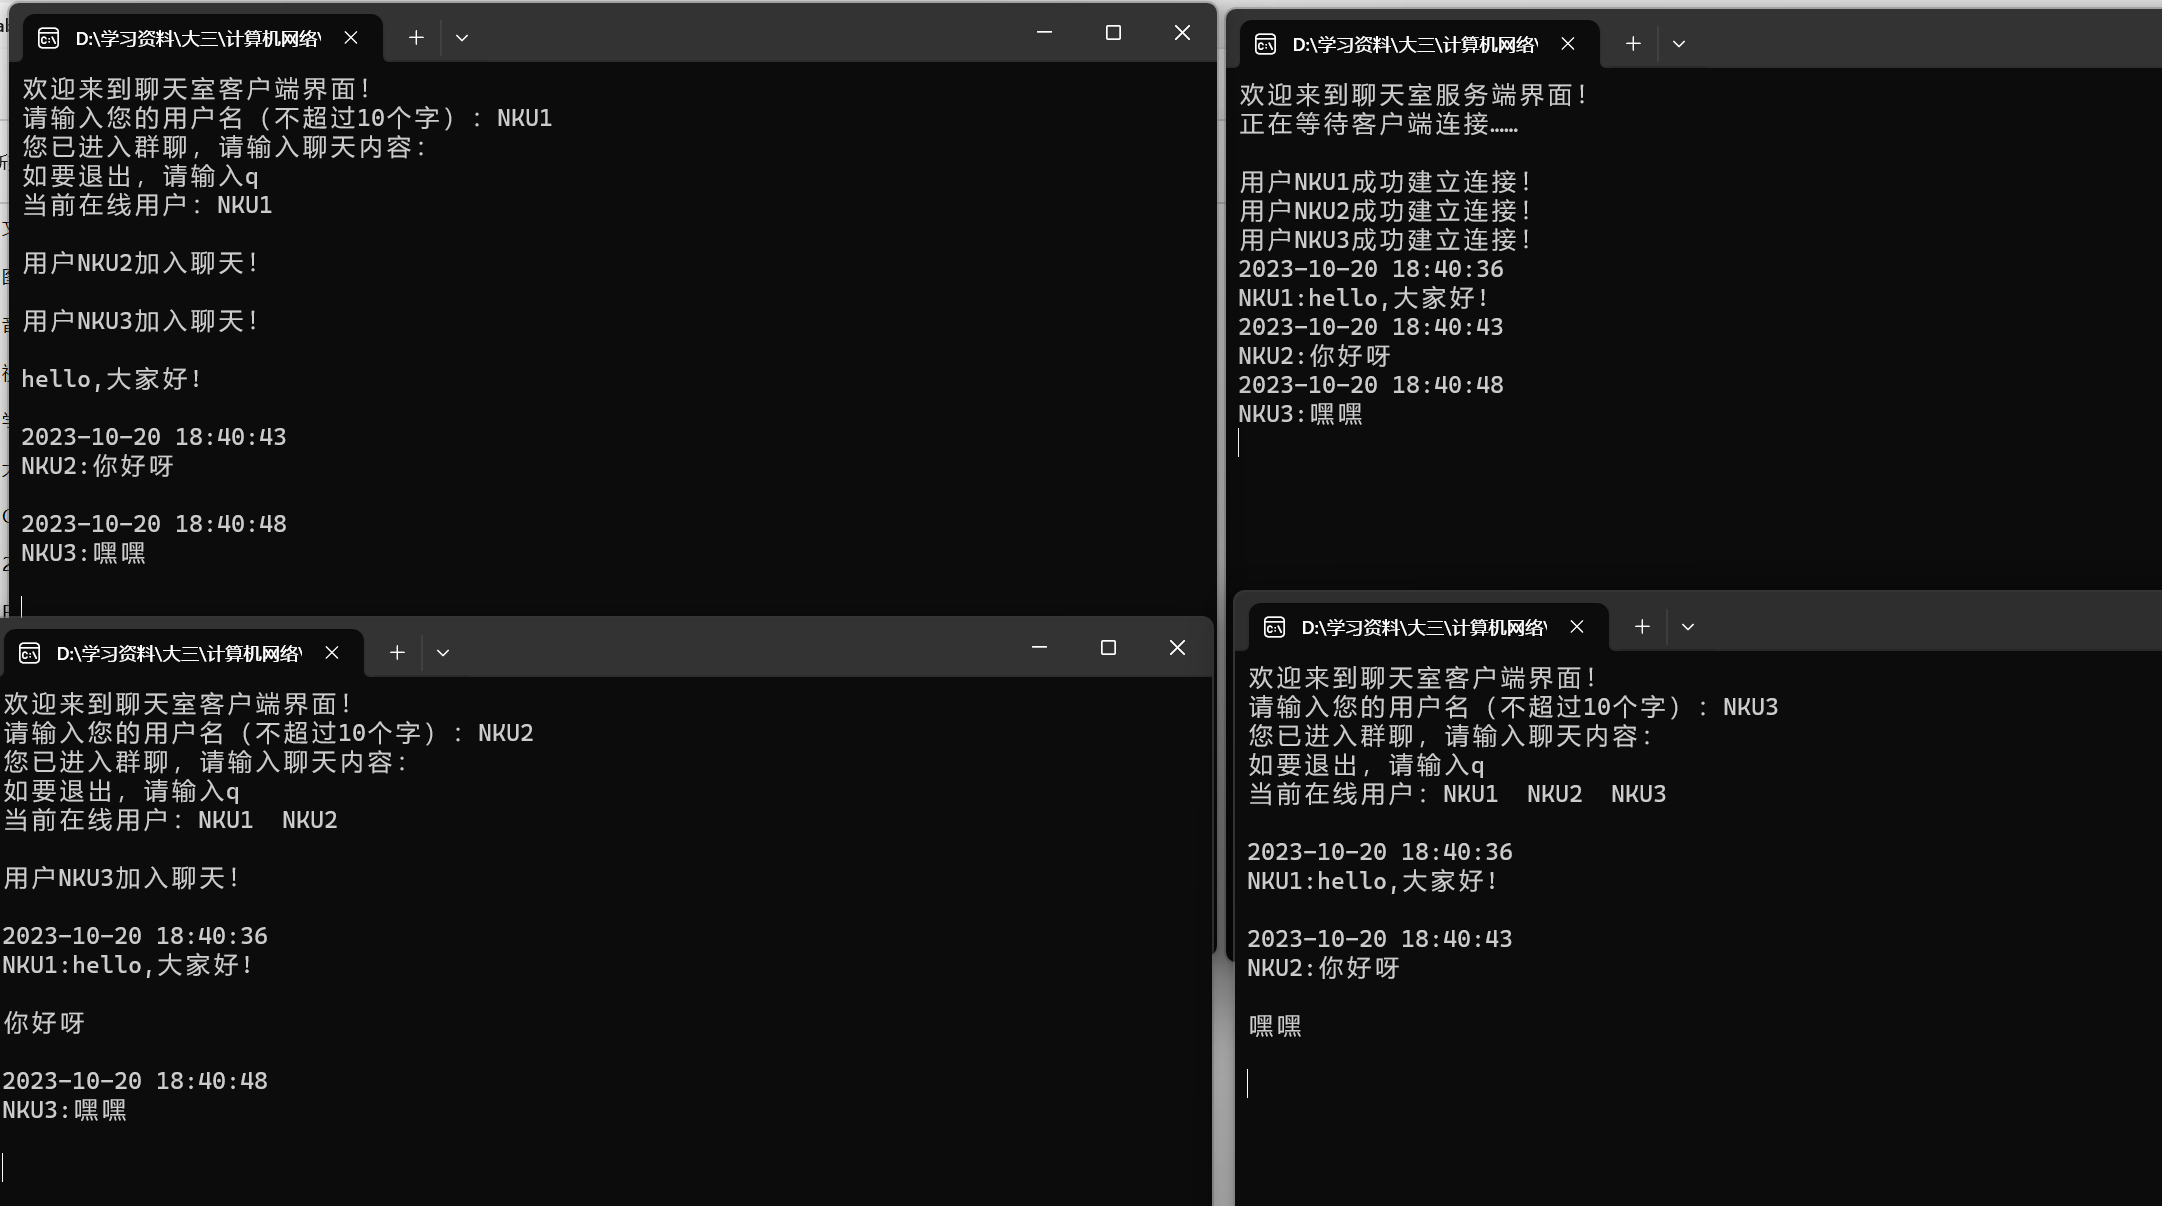
\includegraphics[width=0.8\textwidth]{img/群聊中.png}
    \caption{群聊中}
\end{figure}
NKU3退出后,其他用户可以收到退出信息,服务端也显示NKU3断开连接
\begin{figure}[H]
    \centering
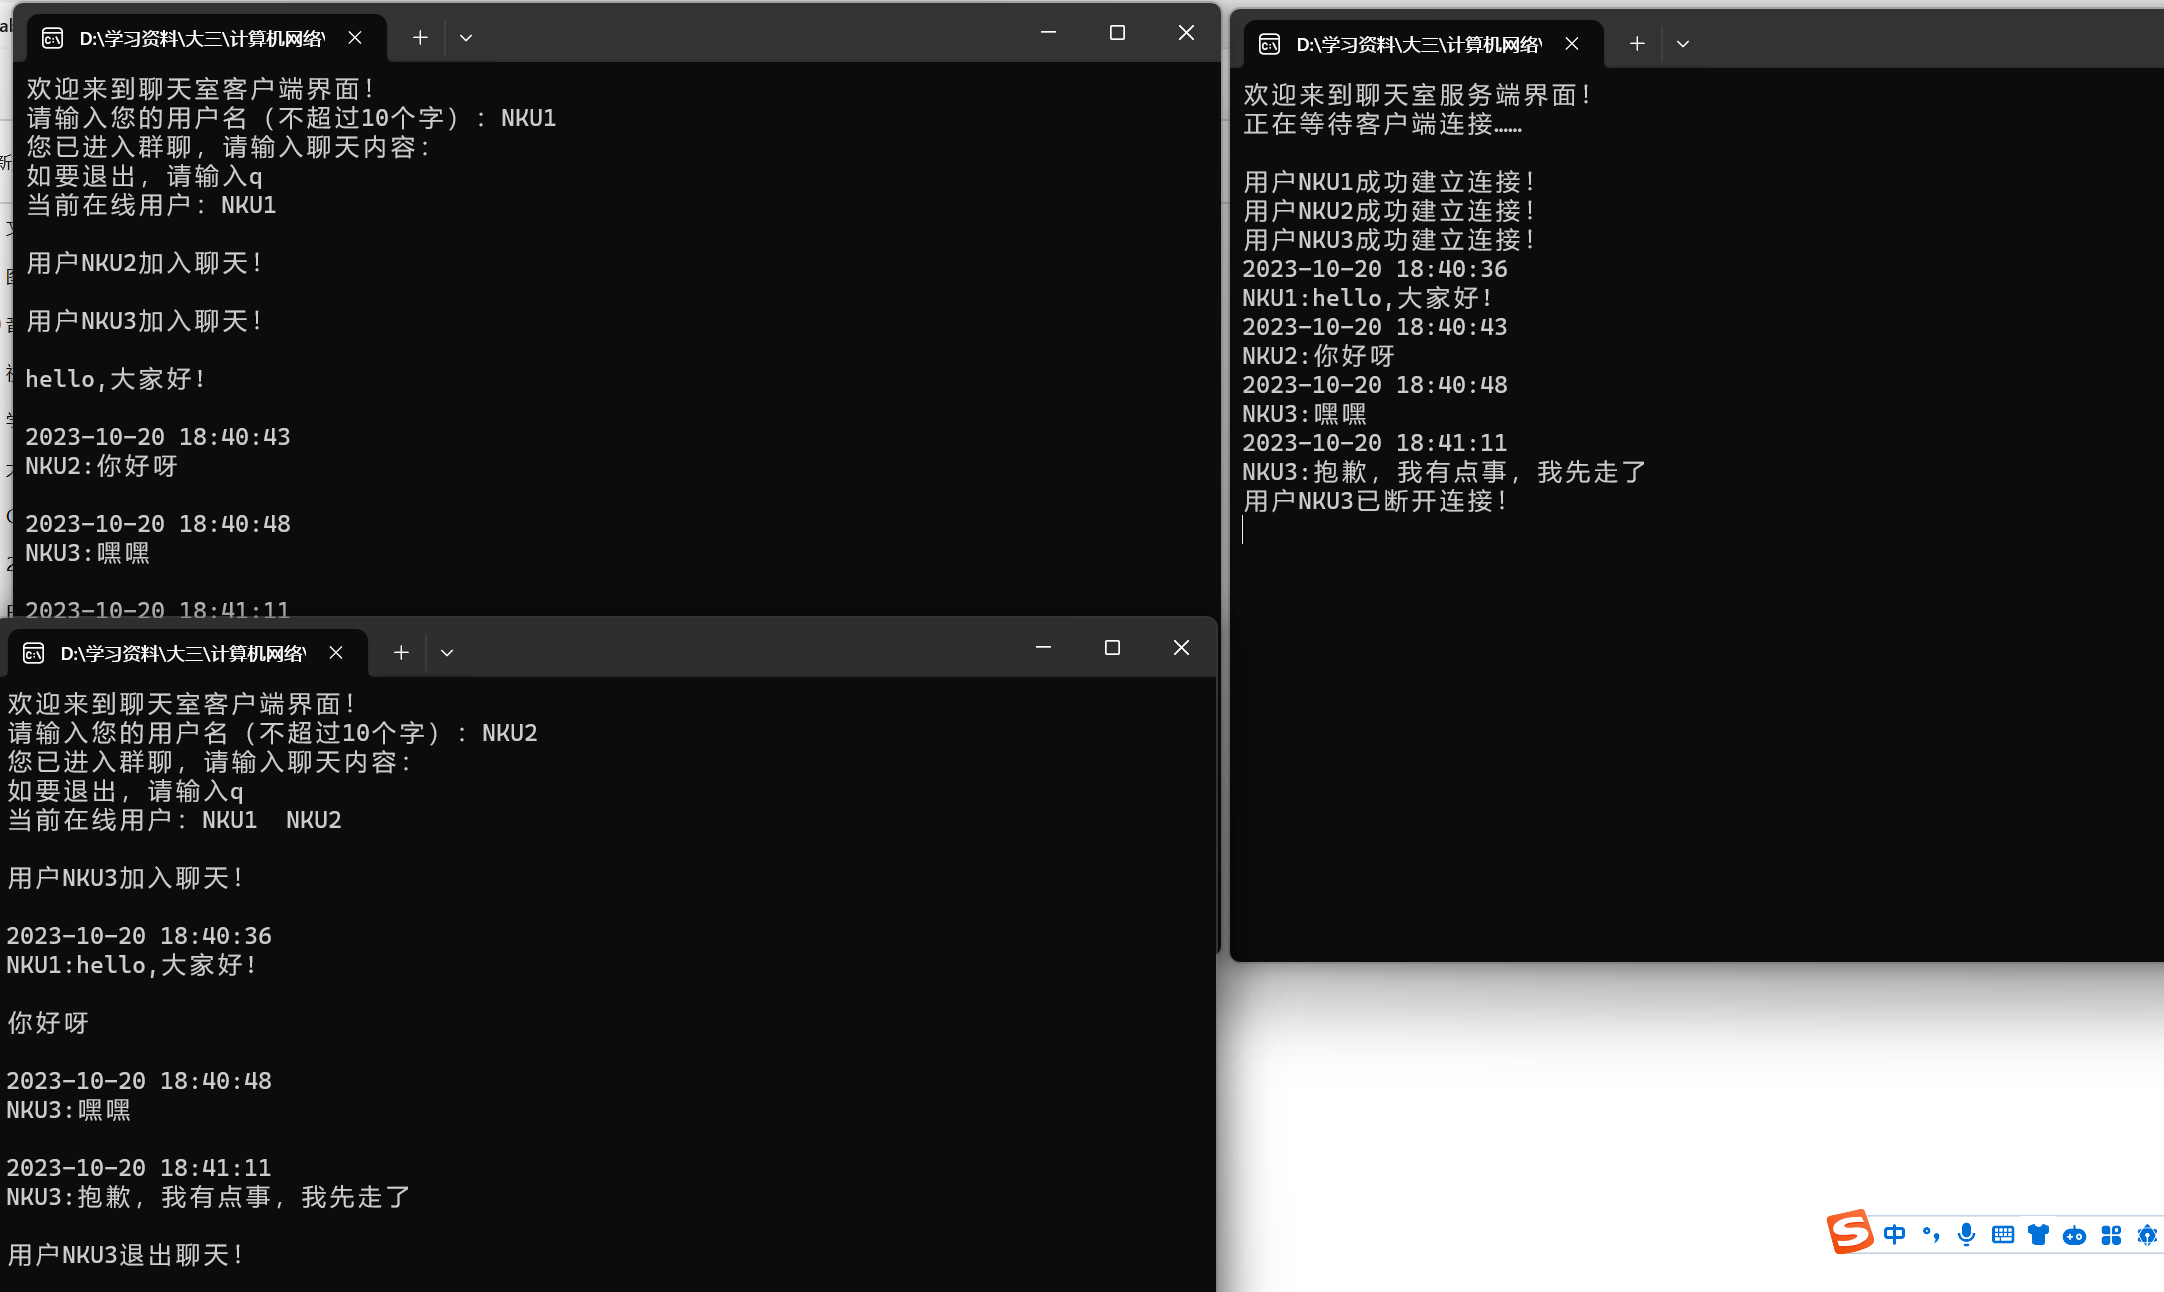
\includegraphics[width=0.8\textwidth]{img/一人退出.png}
    \caption{一人退出}
\end{figure}
所有人退出后,服务端中显示聊天记录和成功/断开连接的记录
\begin{figure}[H]
    \centering
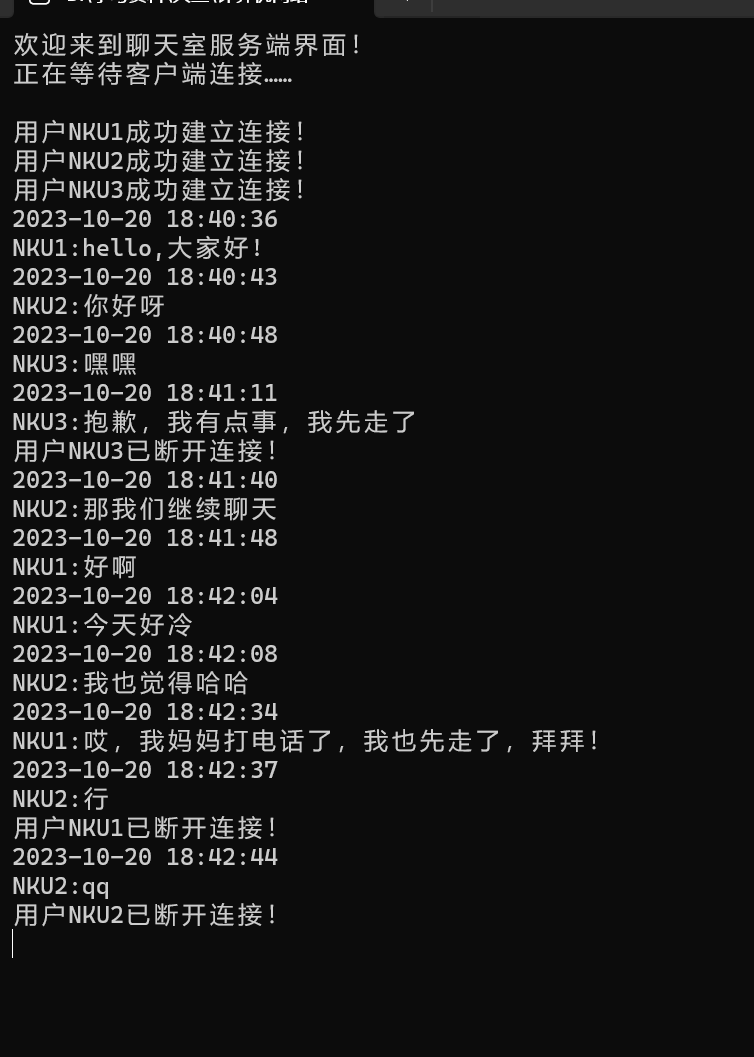
\includegraphics[width=0.4\textwidth]{img/后台记录.png}
    \caption{后台记录}
\end{figure}

\subsection{抓包分析}
下面用WireShark软件对网络通信进行分析,首先打开软件,点击Adapter for loopback traffic capture,用于抓取本地主机(即127.0.0.1或localhost)上的通信数据。
\begin{figure}[H]
    \centering
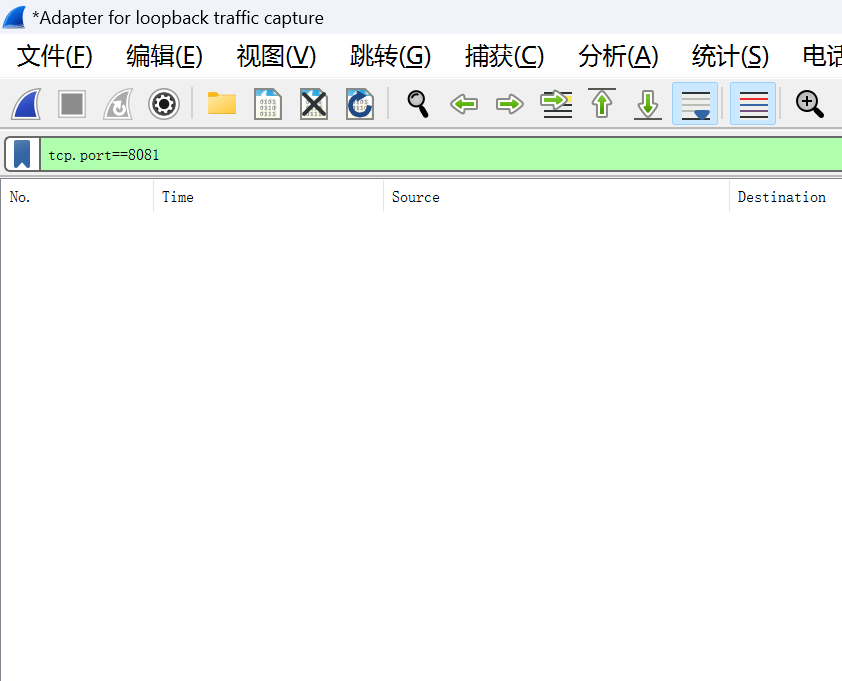
\includegraphics[width=0.4\textwidth]{img/WireShark初始化.png}
    \caption{WireShark初始化}
\end{figure}
打开后,因为在实验中使用TCP协议来进行流式传输,以及服务端端口号为8080,所以设置输出过滤:$tcp.port==8080$
\begin{figure}[H]
    \centering
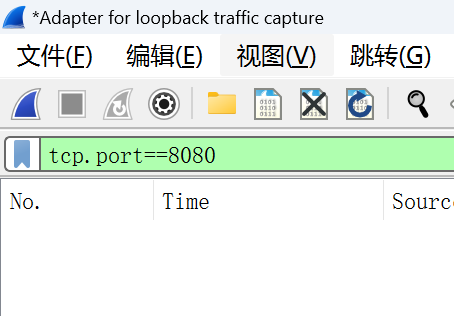
\includegraphics[width=0.4\textwidth]{img/过滤条件.png}
    \caption{过滤条件}
\end{figure}
点击开始捕获后,运行可执行文件,输入第一个用户的名字“NKU1”,按照实验代码,用户端会向服务端传输一个“\$n\$ame:NKU1”的消息,如下图可以看到,已经成功捕获到该消息。另外在图中,我也看到了TCP的三次握手过程,即前三行内容:[SYN]、[SYN,ACK]、[ACK],第四行即是发出的消息。同时根据TCP协议的特点,发送方发送一个带有[PSH, ACK]标志的数据包,接收方收到后会回应一个带有[ACK]标志的数据包,表示已经收到发送的数据。第四、五内容验证了这一特点。而第六行消息则是服务端返回给用户的当前在线用户的消息,第七行则是[ACK]应答,符合预期。通过抓包看到,TCP协议更像是“一问一答”的模式,在实际通信中发送方也在接收接收方回应的数据包。
\begin{figure}[H]
    \centering
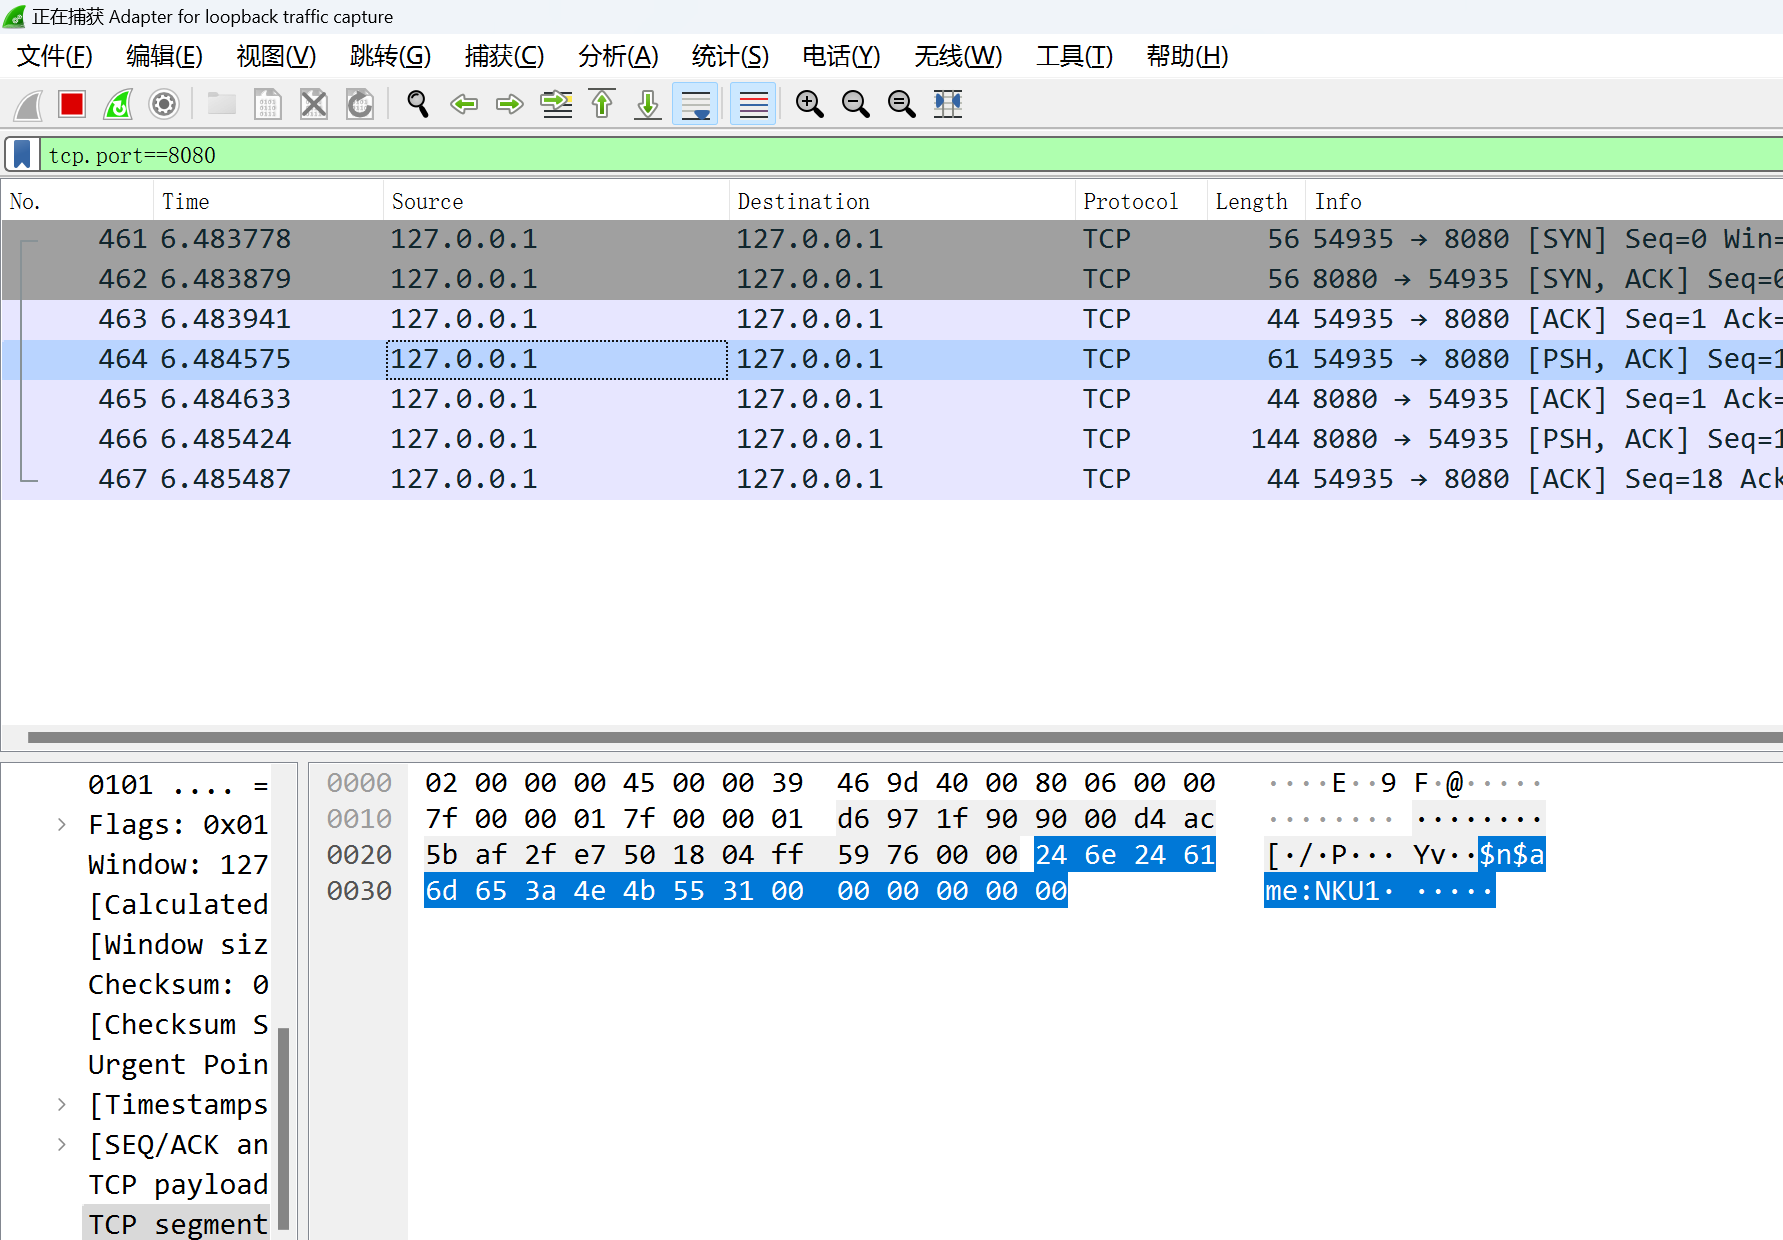
\includegraphics[width=0.8\textwidth]{img/捕获结果.png}
    \caption{捕获结果}
\end{figure}
点开第四行消息查看详细内容,可以看到使用的是IPv4协议,源端口号为54935(这个端口号是操作系统为客户端分配的),目的端口号即为服务端设置的端口号(8080)。
\begin{figure}[H]
    \centering
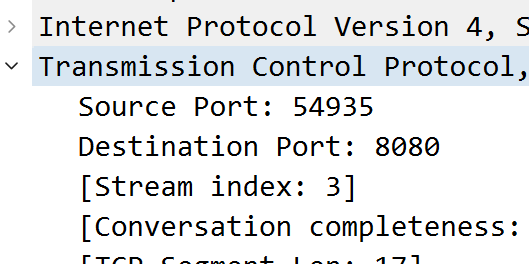
\includegraphics[width=0.5\textwidth]{img/详细信息.png}
    \caption{详细信息}
\end{figure}\par
综上,通过WireShark能够捕获到符合实验预期的通信内容,验证成功。

\section{问题\&解决方案}
在实验过程中,遇到了一系列问题并且最终成功解决\par
\vspace{0.5cm}

 \textbf{问题1}\par
线程的创建以及结束,实验要求使用多线程的方式完成聊天程序。由于对线程的相关知识了解不足,在编写代码时不能正确处理线程函数。在用户端输入q退出线程的时候,用户端主函数return 0 结束线程,但子线程仍在接收服务器发送的内容。会出现recv失败的情况。\par
\vspace{0.2cm}
\textbf{解决}\par
用户端输入q退出时,仍会将q发送给服务端,并且服务端接收到后,以SOCKET套接字为索引,发送给用户端的子线程。子线程接收到q后通过return 0 即可正常退出。

\vspace{0.5cm}
\textbf{问题2}\par
用户端输入名字后,每次发送消息时,可以在用户端把时间、用户名和原始消息封装起来一起发给服务端,但每发送一次就需要读取一次用户名,效率较低。\par
\vspace{0.2cm}
\textbf{解决}\par
用全局链表维护在线用户,用户连接成功后就立即向服务端发送一条包含用户名特殊消息,服务端拿到后把用户名存储在链表中,下次再收到该用户发送的消息时就从链表中获取用户名.


\section{思考总结}
在本次实验中,由于对线程等相关知识还不够熟悉,对线程的处理只考虑了基本的创建和退出功能,没有考虑并发等情况,之后使用多线程方式编程时,会尝试加入互斥量等机制来避免可能出现的问题。通过本次实验,我初步了解了socket编程的编程方式,对理论知识有了更深入的了解,熟悉了如何采用多线程编程,熟悉了如何使用WireShark进行抓包分析,提高了编程能力。
\vspace{0.5cm}

\end{document}
